\begin{figure}[!htbp]
\centering
\caption{Correlation Between Democracy and Outcomes}\label{fig:ols}
\captionsetup{width=0.8\textwidth}
\centering
  \subcaptionbox{GDP Growth Rate in 2020\label{fig:ols-gdp}}{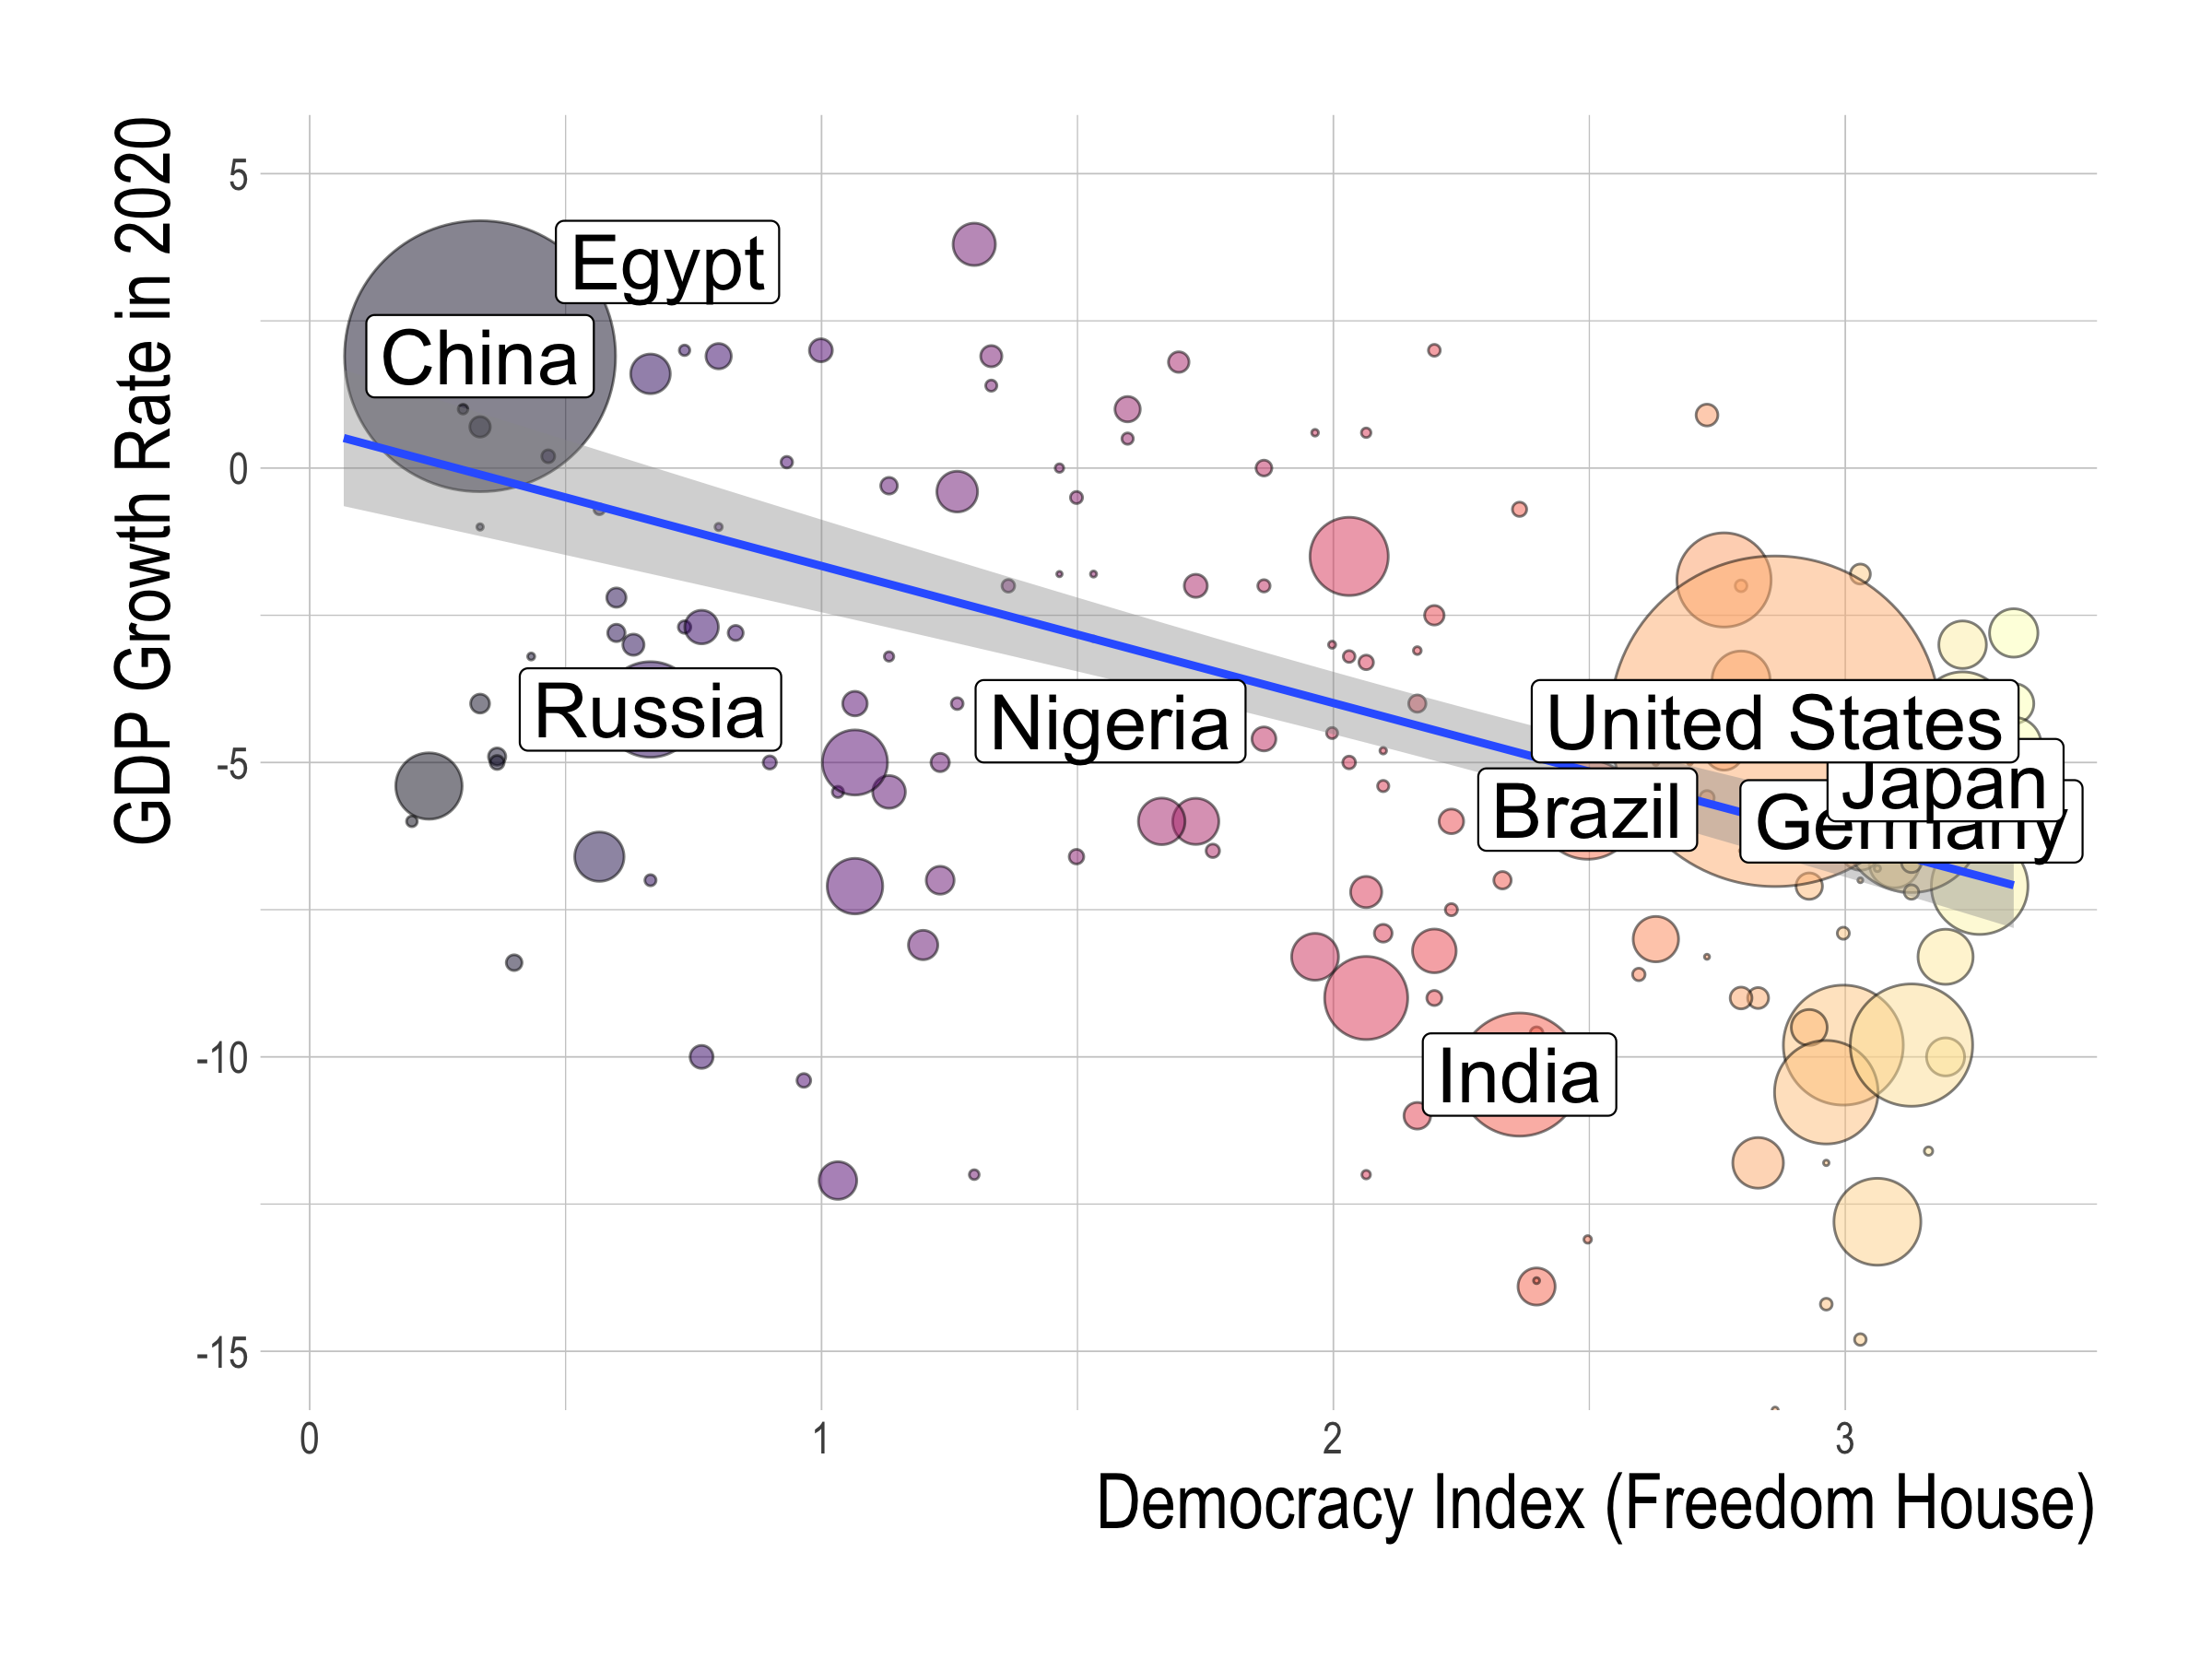
\includegraphics[width=4.4in]{plots/figure1a.png}}
  
  \subcaptionbox{Covid-19-related Deaths Per Million \label{fig:ols-deaths}}{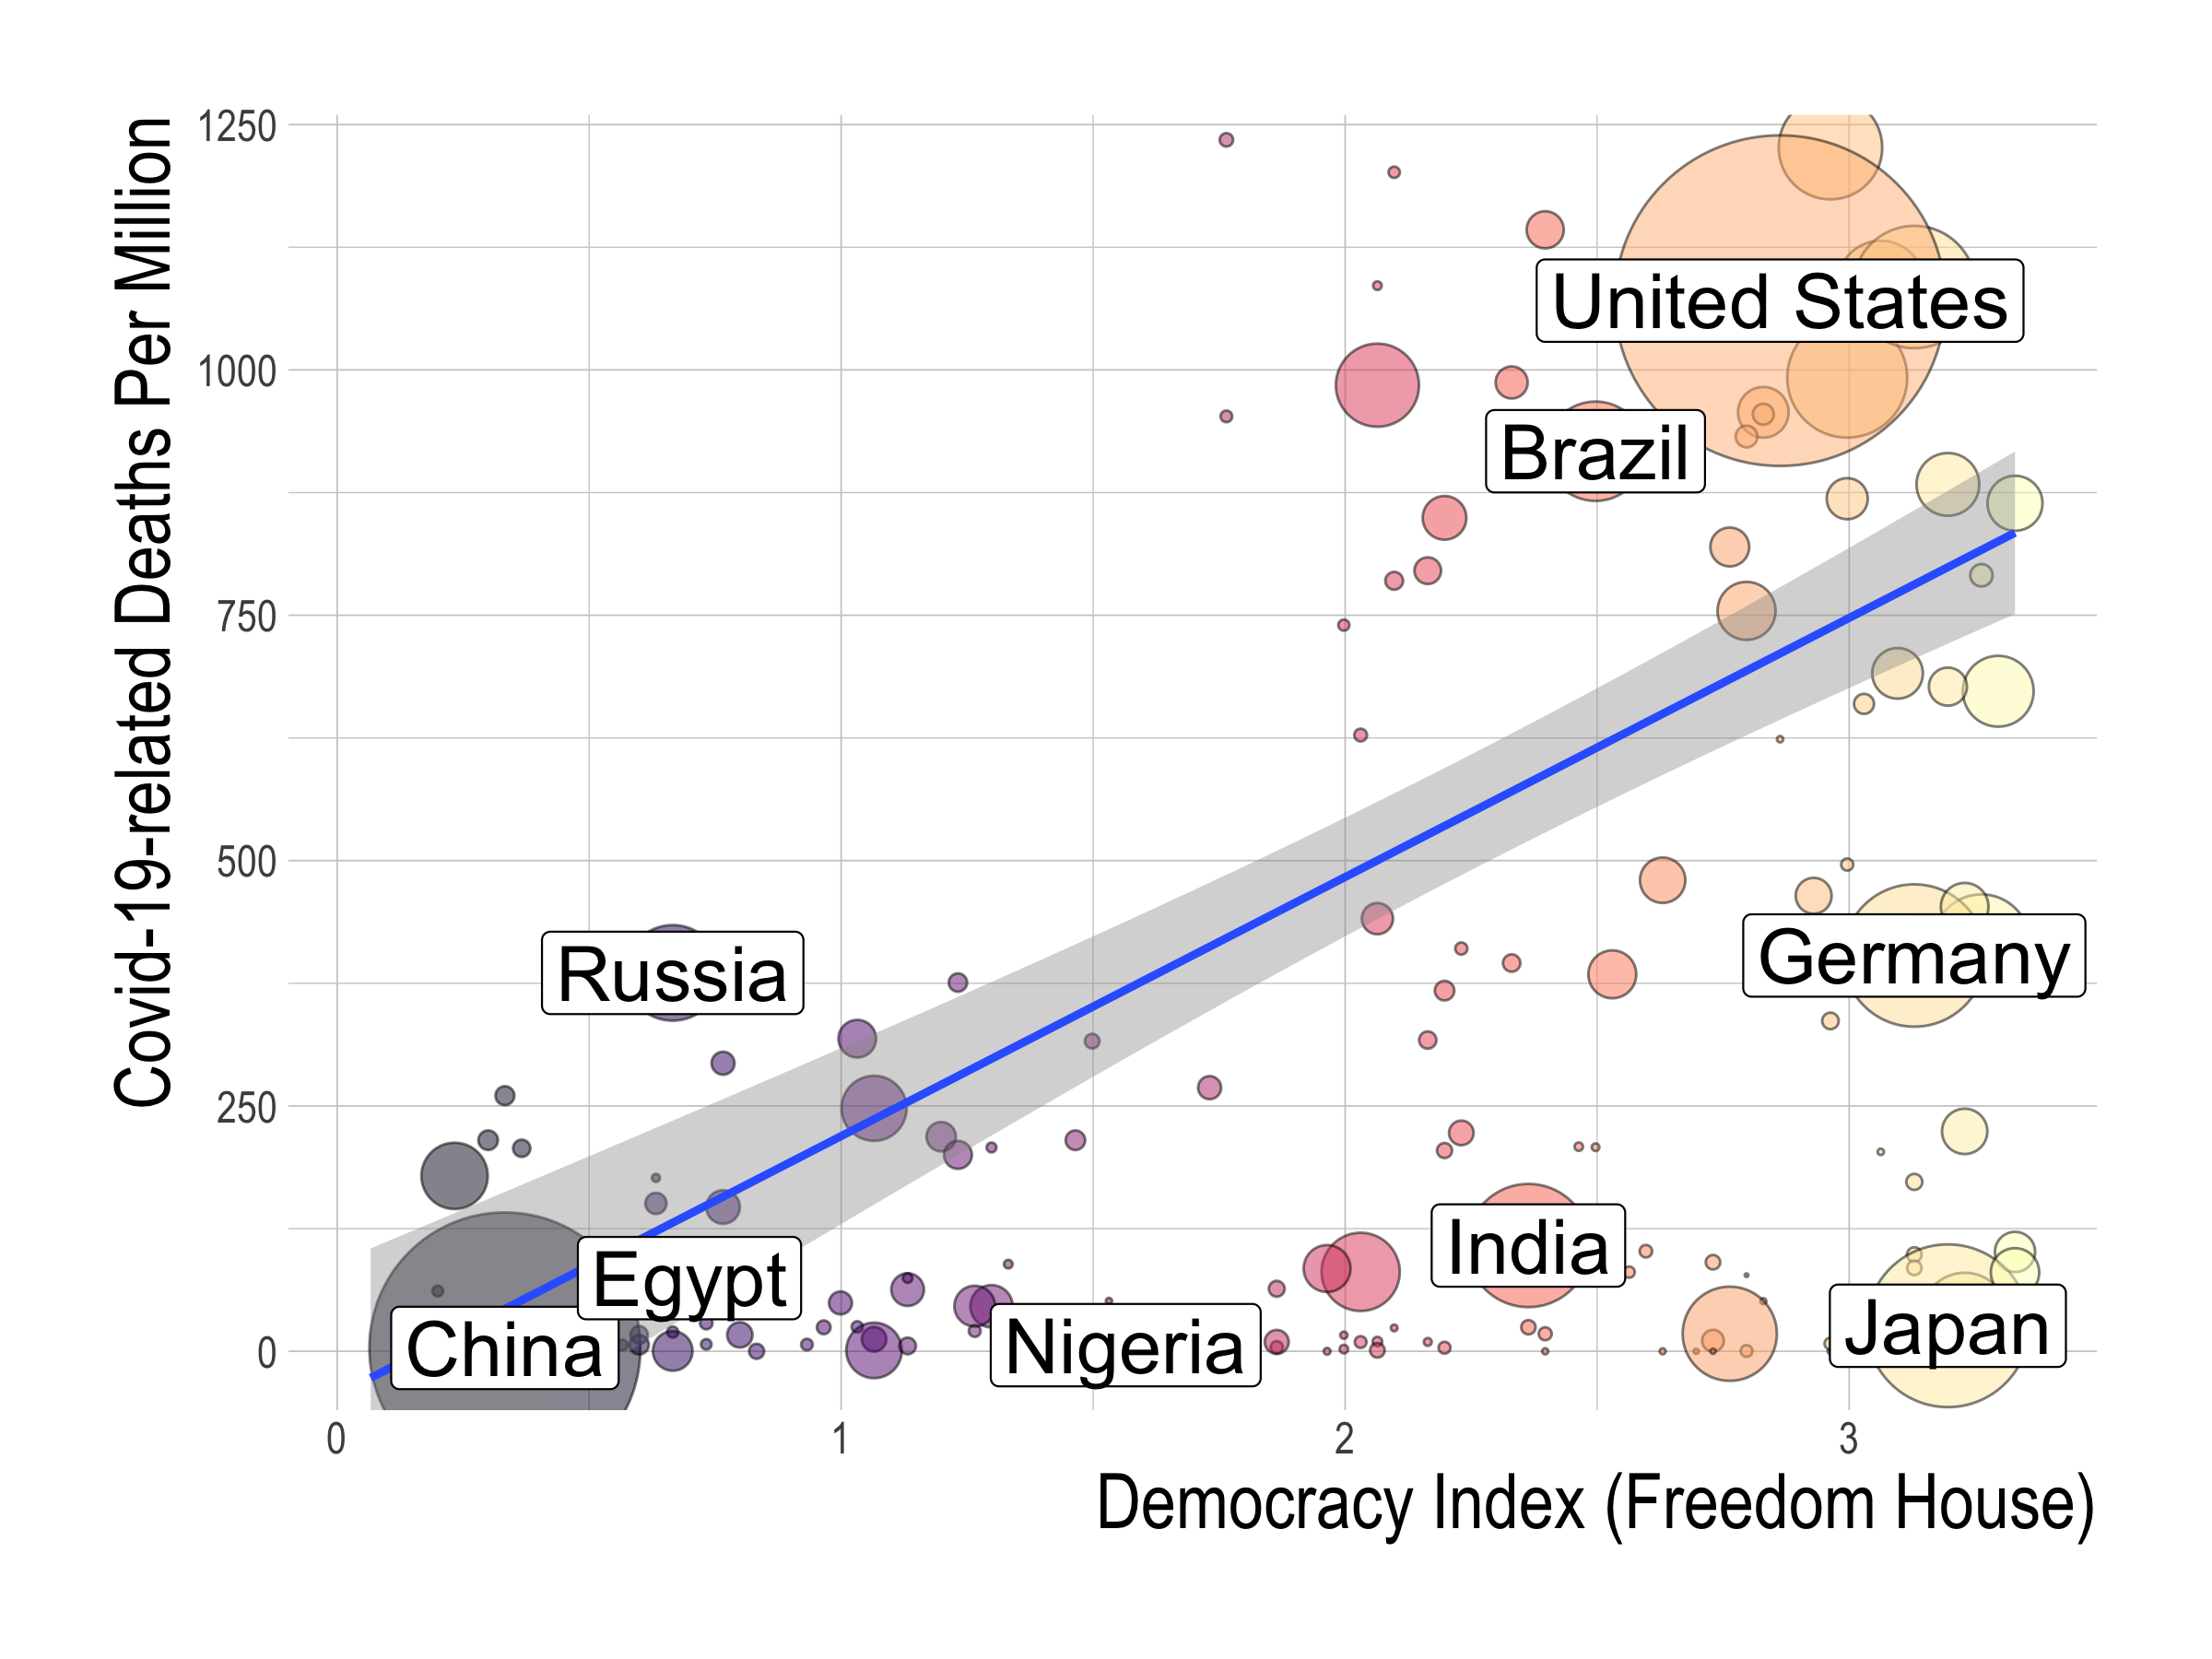
\includegraphics[width=4.4in]{plots/figure1b.png}}
  \caption*{\textit{Notes:} Figure (a) shows the relationship between democracy and GDP growth rates in 2020. Figure (b) shows the relationship between democracy and Covid-19-related deaths per million. The Democracy Index (Freedom House) is the sum of the political rights and civil liberties scales from \emph{Freedom in the World 2020} by Freedom House. It is normalized to have standard deviation one. The size of each observation point is proportional to the country's GDP. The colors depend on the level of the democracy index (warmer colors for democracy and darker colors for autocracies). The line is the fitted line from a univariate OLS regression of Covid-19 outcomes against the democracy index that weights observations by GDP. The shaded area corresponds to the 95\% confidence interval.}
\end{figure}
